\chapter{Requirements}
\section{Allgemeine Beschreibung}
\subsection{Produktperspektive}
Mit Internet of Things sind eine Vielzahl neuartige Devices entstanden. Während in herkömmlichen Netzwerken hauptsächlich Personal Computer, Notebooks, Server usw. verwaltet werden mussten, so bringen IoT Devices den IT-Abteilungen neue Herausforderungen. Zum einen dürfte die Anzahl Geräte gegenüber herkömmlichen Computer deutlich ansteigen, zum anderen sind IoT Devices in Sachen Funktionalität und Rechenleistung, sowie auch der Netzwerkbandbreite deutlich beschränkt. 

Mit dieser Arbeit soll eine Management Applikation bereitgestellt werden, um eine Vielzahl unterschiedlicher IoT Devices administrieren zu können. 
\subsection{Produkfunktionen}
Die Applikation soll den Benutzern erlauben, IoT Geräte zu verwalten. Die Aufgaben reichen vom Erfassen und Discovery von Devices über die Konfigurationsverwaltung und Softwareverteilung bis zu Backup und Restore. Ausserdem sollen Management-relevante Kommandos auf Devices ausgeführt- und Security Aspekte beachtet werden. Die Details zu den Produktfunktionen sind den Use Cases zu entnehmen.

\subsection{Benutzer Charakteristik}
Zielpersonen der Applikation sind Betreiber von IoT Devices. Dies können im Enterprise Umfeld IT-Mitarbeiter in operationeller Funktion-, oder auch Softwareentwickler für IoT Applikationen sein. Heimanwender können bei entsprechenden Kenntnissen ebenfalls zur Zielgruppe gehören. Es werden solide Grundkenntnisse in TCP/IP Netzwerken sowie Verständnis der verwendeten IoT Architekturen und Devices vorausgesetzt. 
\subsection{Einschränkungen}
Eventuelle Einschränkungen werden in der Designphase noch genauer spezifiziert. Momentan gibt es noch keine spezifische Einschränkungen
\section{Use Cases}
\subsection{Use Cases Diagramm}
\begin{figure}[H]
\centering
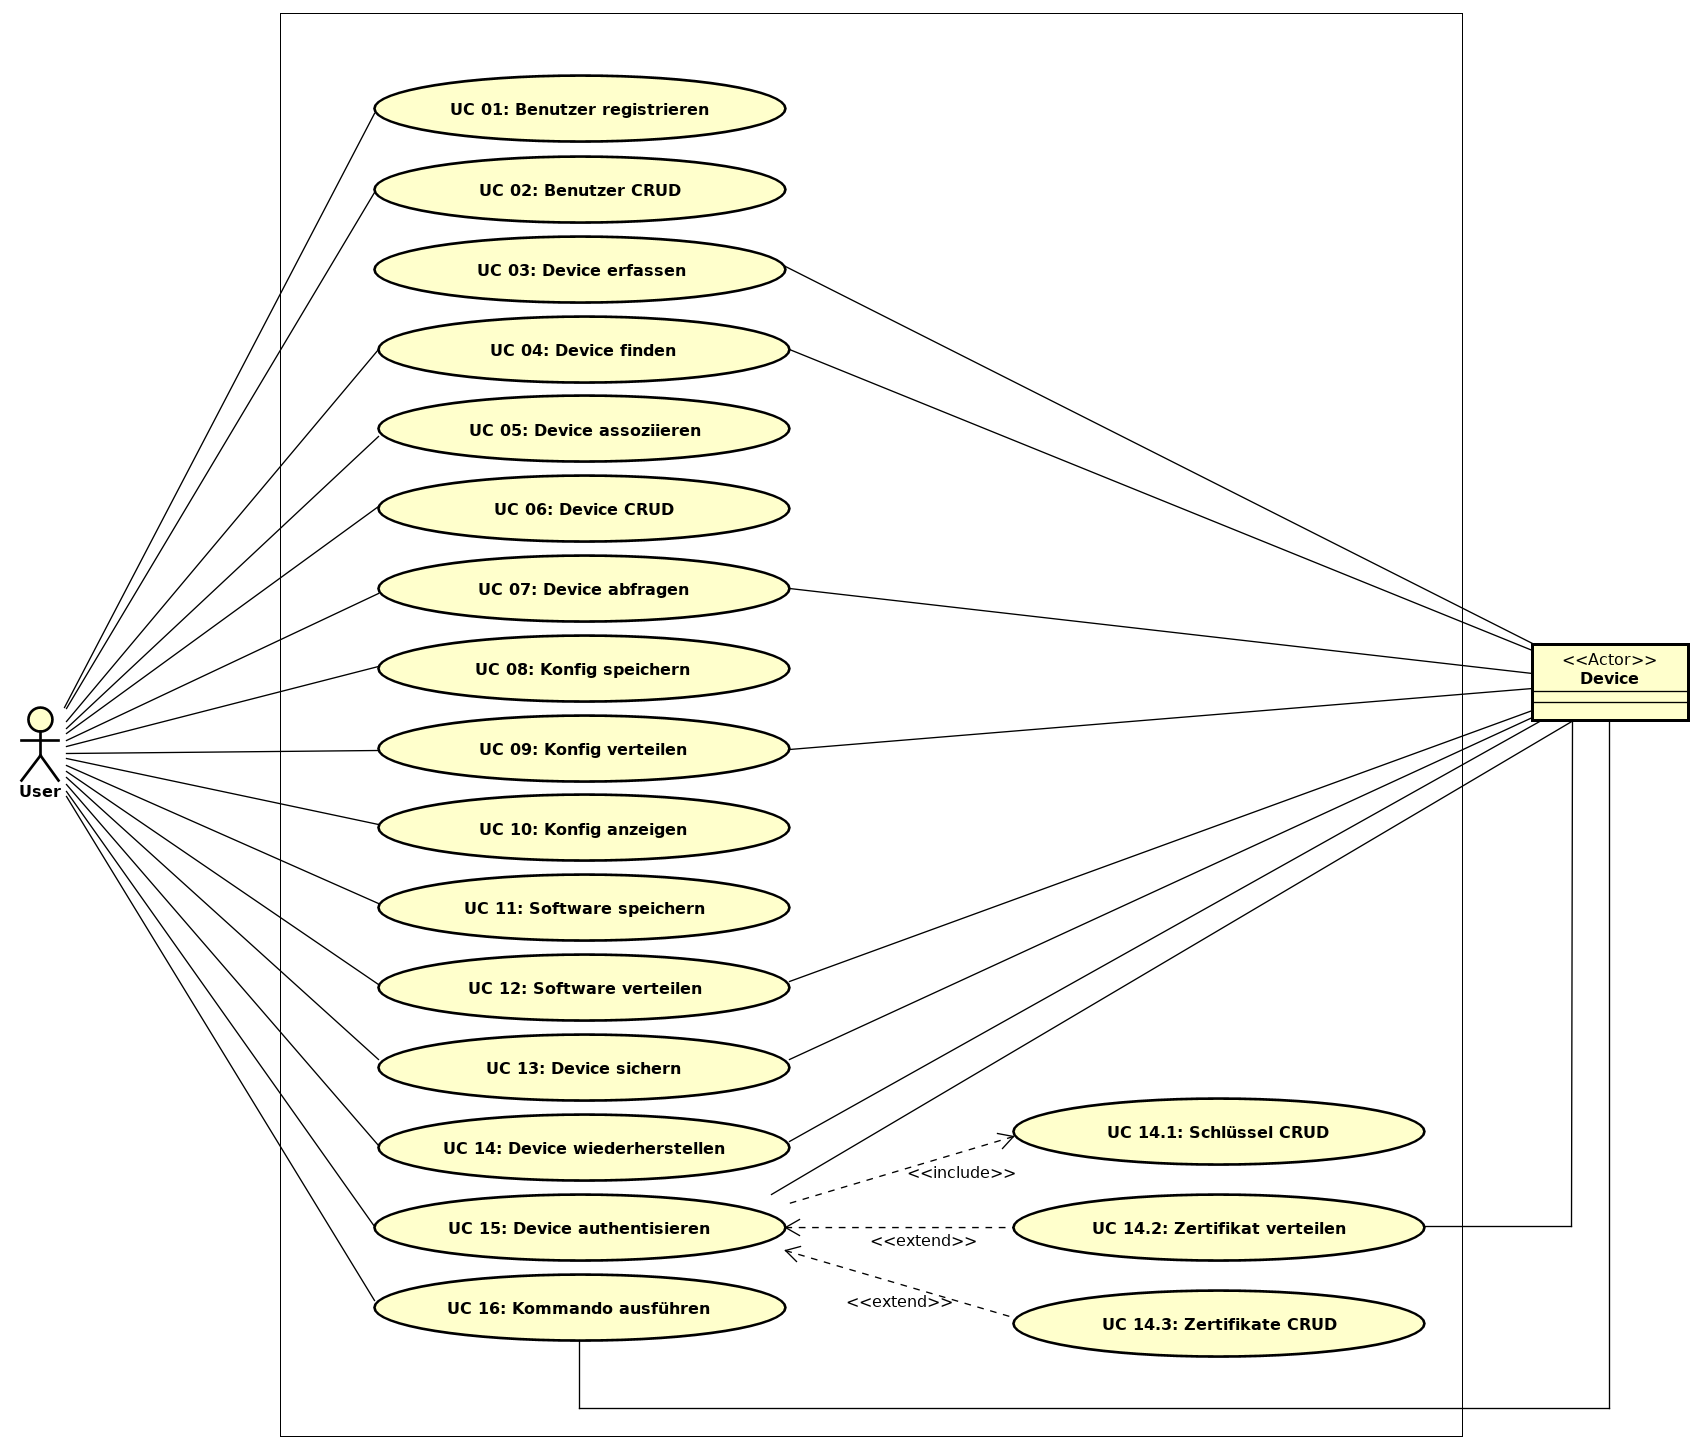
\includegraphics[scale=0.39]{images/use_case_diagram.png}\caption{Use Case Diagramm}
\end{figure}
\newpage
\subsection{Priorisierung}
Da die Umsetzung aller Use Cases den Rahmen einer Bachelorarbeit sprengen würde, wurden die diese wie folgt priorisiert:
\begin{center}
\begin{longtable}{| p{5.5cm} | p{3cm} |}
\hline
\textbf{Use Case} & \textbf{Priorität}\\ \hline
UC 01: Benutzer registrieren     & Optional \\ \hline
UC 02: Benutzer CRUD	         & Optional \\ \hline 
UC 03: Device erfassen           & Pflicht \\ \hline 
UC 04: Device finden             & Pflicht \\ \hline 
UC 05: Device assoziieren        & Pflicht \\ \hline 
UC 06: Device CRUD               & Pflicht \\ \hline 
UC 07: Device abfragen           & Pflicht \\ \hline 
UC 08: Konfig speichern          & Pflicht \\ \hline 
UC 09: Konfig verteilen          & Optional \\ \hline 
UC 10: Konfig anzeigen           & Pflicht \\ \hline 
UC 11: Software speichern        & Pflicht \\ \hline 
UC 12: Software verteilen        & Optional \\ \hline 
UC 13: Device sichern            & Optional \\ \hline 
UC 14: Device wiederherstellen   & Optional \\ \hline 
UC 15: Device authentisieren     & Optional \\ \hline 
UC 15.1: Schlüssel CRUD          & Pflicht \\ \hline 
UC 15.2: Zertifikat verteilen    & Optional \\ \hline 
UC 15.3: Zertifikat CRUD         & Pflicht \\ \hline 
UC 16: Kommando ausführen        & Pflicht \\ \hline 
\end{longtable}
\end{center}
\subsection{Aktoren}
Der Benutzer der Applikation ist in diesem System der einzige primäre Aktor. Dieser bewirtschaftet die Applikation und verwaltet alle Devices und Benutzer. Als Sekundärer Aktor werden die einzelnen Devices gezählt.
\newpage
\subsection{Beschreibungen (Casual)}
\subsubsection{Benutzer registrieren}
\mbox{}
\begin{longtable}{| p{4cm} | p{11.7cm} |}
 \hline
 \textbf{ID} & 01\\ \hline 
 \textbf{Name} & Benutzer registrieren\\ \hline 
 \textbf{Beschreibung} & Der Benutzer legt sich einen neuen Account für die Management Software an.\\ \hline 
 \textbf{Preconditions} & 
   \tabitem Applikation gestartet
  \\ \hline 
 \textbf{Postconditions} & 
  \tabitem Neuer Benutzer ist gespeichert
 \\ \hline
 \textbf{Main Success Scenario} &
 1. Benutzer wählt ''Benutzer registrieren'' \newline
 2. Benutzer gibt Loginangaben ein \newline
 3. Benutzer speichert die Eingaben
\\  \hline 
 \textbf{Extensions} & -\\ \hline 
 \end{longtable}

\subsubsection{Benutzer CRUD}
\mbox{}
\begin{longtable}{| p{4cm} | p{11.7cm} |}
 \hline
 \textbf{ID} & 02\\ \hline 
 \textbf{Name} & Benutzer CRUD\\ \hline 
 \textbf{Beschreibung} & Benutzerverwaltung der Applikation\\ \hline 
 \textbf{Preconditions} & 
   \tabitem Applikation gestartet \newline
   \tabitem Benutzer ist registriert \newline
   \tabitem Benutzer ist eingeloggt 
  \\ \hline 
 \textbf{Postconditions} & 
  \tabitem Änderungen gespeichert
 \\ \hline
 \textbf{Main Success Scenario} &
 \textbf{Create:}\newline
  1. UC 01: Benutzer registrieren \newline
 \textbf{Read:}\newline
  1. Benutzer lässt Userdaten anzeigen \newline
 \textbf{Update:}\newline
  1. Benutzer lässt Userdaten anzeigen \newline
  2. Benutzer verändert Attribute\newline
  3. Benutzer speichert Änderungen\newline
 \textbf{Delete:}\newline
  1. Benutzer wird gelöscht \\ 
 \hline 
 \textbf{Extensions} & -\\ \hline 
 \end{longtable}
\newpage
\subsubsection{Device erfassen}
\mbox{}
\begin{longtable}{| p{4cm} | p{11.7cm} |}
 \hline
 \textbf{ID} & 03\\ \hline 
 \textbf{Name} & Device erfassen \\ \hline 
 \textbf{Beschreibung} & Der Benutzer möchte ein Device manuell hinzufügen. Der Endpunkt ist dem Benutzer bekannt. 
 \\ \hline 
 \textbf{Preconditions} & 
   \tabitem Applikation gestartet \newline
   \tabitem Benutzer eingeloggt \newline
   \tabitem Device Endpunkt ist dem Benutzer bekannt
  \\ \hline 
 \textbf{Postconditions} & 
  \tabitem Falls ein Gerät gefunden wird, wird es angezeigt 
  \\ \hline 
 \textbf{Main Success Scenario} & 
  1. Benutzer öffnet Device Erfassung \newline
  2. Benutzer gibt Device Endpunkt ein \newline
  3. Benutzer startet Suchvorgang \newline
  4. Anfrage wird an Device gesendet \newline
  5. Antwort vom Device wird angezeigt
 \\ \hline 
 \textbf{Extensions} & 
  5.a Timeout Fehlermeldung wird dem Benutzer angezeigt 
  \\ \hline 
\end{longtable}
\subsubsection{Device finden}
\mbox{}
\begin{longtable}{| p{4cm} | p{11.7cm} |}
 \hline
 \textbf{ID} & 04\\ \hline 
 \textbf{Name} & Device finden\\ \hline 
 \textbf{Beschreibung} & Der Benutzer möchte ein- oder meherere Devices finden. Endpunkt des Devices ist dem Benutzer unbekannt. Gefundene Devices sollen dem Benutzer aufgelistet werden. \\ \hline 
 \textbf{Preconditions} &  
  \tabitem Applikation gestartet \newline
  \tabitem Benutzer eingeloggt
 \\ \hline 
 \textbf{Postconditions} & 
  \tabitem Gefundene Devices werden dem Benutzer angezeigt 
 \\ \hline 
 \textbf{Main Success Scenario} & 
  1. Benutzer öffnet Device Discovery \newline
  2. System listet eingegangene Anfragen von Devices auf \newline
 \\ \hline 
 \textbf{Extensions} &  
  2.a System zeigt Fehlermeldung an
 \\ \hline 
 \end{longtable}
\subsubsection{Device assoziieren}
\mbox{}
\begin{longtable}{| p{4cm} | p{11.7cm} |}
 \hline
 \textbf{ID} & 05\\ \hline 
 \textbf{Name} & Device assoziieren \\ \hline 
 \textbf{Beschreibung} & Der Benutzer möchte ein Device verwalten. Dazu muss er das gefundene Device in das System adoptieren.   \\ \hline 
 \textbf{Preconditions} & 
  \tabitem Applikation gestartet \newline
  \tabitem Benutzer eingeloggt \newline
  \tabitem Mindestens 1 Device gefunden 
 \\ \hline 
 \textbf{Postconditions} & 
  \tabitem Assoziation zu gefundenem Device erstellt
 \\ \hline 
 \textbf{Main Success Scenario} &
  1. Benutzer selektiert ein gefundenes Device aus.(UC 03 / UC 04)
  2. Benutzer wählt ''Device adoptieren'' aus
  3. Assoziation wird im System eingetragen 
 \\ \hline 
 \textbf{Extensions} & -\\ \hline 
 \end{longtable}
\newpage
\subsubsection{Device CRUD}
\mbox{}
\begin{longtable}{| p{4cm} | p{11.7cm} |}
 \hline
 \textbf{ID} & 06\\ \hline 
 \textbf{Name} & Device CRUD\\ \hline 
 \textbf{Beschreibung} & Deviceverwaltung der Applikation\\ \hline 
 \textbf{Preconditions} & 
  \tabitem Applikation gestartet \newline
  \tabitem Benutzer eingeloggt
 \\ \hline 
 \textbf{Postconditions} & 
  \tabitem Änderungen gespeichert 
 \\ \hline 
 \textbf{Main Success Scenario} &
 \textbf{Create:}\newline
  1. UC 05: Device assoziieren \newline
 \textbf{Read:}\newline
  1. Attribute eines Devices anzeigen \newline
 \textbf{Update:}\newline
  1. Benutzer lässt Device Attribute anzeigen \newline
  2. Benutzer verändert Attribute\newline
  3. Benutzer speichert Änderungen\newline
 \textbf{Delete:}\newline
  1. Device Assoziation wird gelöscht 
  \\ \hline 
 \textbf{Extensions} & -\\ \hline 
 \end{longtable}
 
\subsubsection{Device abfragen}
\mbox{}
\begin{longtable}{| p{4cm} | p{11.7cm} |}
 \hline
 \textbf{ID} & 07\\ \hline 
 \textbf{Name} & Device abfragen\\ \hline 
 \textbf{Beschreibung} & Gewünschte Parameter und Attribute werden vom Device abgefragt\\ \hline 
 \textbf{Preconditions} &  
  \tabitem Applikation gestartet \newline
  \tabitem Benutzer eingeloggt 
 \\ \hline 
 \textbf{Postconditions} & 
  \tabitem Antwort vom Device oder Fehlermeldung wird angezeigt 
 \\ \hline 
 \textbf{Main Success Scenario} & 
  1. Benutzer wählt Device aus \newline
  2. Benutzer startet Abfrage \newline
  3. System sendet Anfrage an Device \newline
  4. System speichert Antwort (UC 06: Device CRUD)
 \\ \hline 
 \textbf{Extensions} & 
  1.a Benutzer wählt mehrere Devices aus \newline
  3.a System sendet Anfragen an mehrere Devices \newline
  3.b Timeout-Fehlermeldung
 \\ \hline 
 \end{longtable}
\newpage
\subsubsection{Konfiguration speichern}
\mbox{}
\begin{longtable}{| p{4cm} | p{11.7cm} |}
 \hline
 \textbf{ID} & 08\\ \hline 
 \textbf{Name} & Konfiguration speichern\\ \hline 
 \textbf{Beschreibung} &  Konfigurationen von beliebigen Devices können im System gespeichert werden\\ \hline 
 \textbf{Preconditions} &
  \tabitem Applikation gestartet \newline
  \tabitem Benutzer eingeloggt \newline
  \tabitem Konfigurationsfile für Benutzer zugänglich   
 \\ \hline 
 \textbf{Postconditions} & 
  \tabitem Konfigurationsfile im System gespeichert
 \\ \hline 
 \textbf{Main Success Scenario} & 
  1. Benutzer wählt ''Upload Konfiguration'' \newline
  2. Benutzer wählt via File-Explorer eine Konfigurationsdatei aus \newline
  3. Konfigurationsdatei hochgeladen \newline
  4. Feedback an den Benutzer, dass die Datei erfolgreich hochgeladen ist.
 \\ \hline 
 \textbf{Extensions} &
  3.a I/O Fehler wird angezeigt \newline
  3.b Timeout-Fehler wird angezeigt 
 \\ \hline 
 \end{longtable}
 
\subsubsection{Konfiguration verteilen}
\mbox{}
\begin{longtable}{| p{4cm} | p{11.7cm} |}
 \hline
 \textbf{ID} & 09\\ \hline 
 \textbf{Name} & Konfiguration verteilen\\ \hline 
 \textbf{Beschreibung} & Konfigurationen können an Devices versendet werden.\\ \hline 
 \textbf{Preconditions} &  
  \tabitem Applikation gestartet \newline
  \tabitem Benutzer eingeloggt \newline
  \tabitem Konfiguration im System vorhanden 
 \\ \hline 
 \textbf{Postconditions} & Konfiguration an Device geschickt\\ \hline 
 \textbf{Main Success Scenario} & 
  1. Benutzer wählt Device aus \newline
  2. Benutzer wählt Konfiguration aus \newline
  3. Benutzer versendet Konfiguration \newline
  4. System zeigt Antwort des Devices an 
 \\ \hline 
 \textbf{Extensions} &
  1.a Benutzer wählt mehrere Device aus \newline
  4.a System zeigt Antworten mehrerer Devices an \newline
  4.b Fehlermeldung wird angezeigt \newline
  4.c Timeout-Fehlermeldung
 \\ \hline 
 \end{longtable}
 
\subsubsection{Konfiguration anzeigen}
\mbox{}
\begin{longtable}{| p{4cm} | p{11.7cm} |}
 \hline
 \textbf{ID} & 10\\ \hline 
 \textbf{Name} & Konfiguration anzeigen\\ \hline 
 \textbf{Beschreibung} & Konfigurationsdetails im System können angesehen werden\\ \hline 
 \textbf{Preconditions} &  
  \tabitem Applikation gestartet \newline
  \tabitem Benutzer eingeloggt \newline
  \tabitem Konfiguration im System vorhanden 
 \\ \hline 
 \textbf{Postconditions} & 
  \tabitem Konfigurationsdetails angezeigt 
 \\ \hline 
 \textbf{Main Success Scenario} &  
  1. Benutzer wählt Konfiguration aus \newline
  2. System zeigt Konfiguration an 
 \\ \hline 
 \textbf{Extensions} & -\\ \hline 
 \end{longtable}
 
\subsubsection{Software speichern}
\mbox{}
\begin{longtable}{| p{4cm} | p{11.7cm} |}
 \hline
 \textbf{ID} & 11\\ \hline 
 \textbf{Name} & Software speichern\\ \hline 
 \textbf{Beschreibung} & Spezifische Software oder Firmware für Devices können im System gespeichert werden.\\ \hline 
 \textbf{Preconditions} &
  \tabitem Applikation gestartet \newline
  \tabitem Benutzer eingeloggt \newline
  \tabitem Softwarefile für Benutzer zugänglich 
 \\ \hline 
 \textbf{Postconditions} & 
  \tabitem Softwarefile im System gespeichert \newline
  1. Benutzer wählt ''Upload Software'' \newline
  2. Benutzer wählt via File-Explorer eine Softwaredatei aus \newline
  3. Softwaredatei hochgeladen \newline
  4. Feedback an den Benutzer, dass die Datei erfolgreich hochgeladen ist.
 \\ \hline 
 \textbf{Extensions} &
  3.a I/O Fehler wird angezeigt
  3.b Timeout-Fehler wird angezeigt 
 \end{longtable}
 
\subsubsection{Software verteilen}
\mbox{}
\begin{longtable}{| p{4cm} | p{11.7cm} |}
 \hline
 \textbf{ID} & 12\\ \hline 
 \textbf{Name} & Software verteilen\\ \hline 
 \textbf{Beschreibung} & Jedes Device hat einen gewissen Softwarestand. Dieser kann durch neue Software ersetzt oder gepatched werden. \\ \hline 
 \textbf{Preconditions} & 
  \tabitem Applikation gestartet\newline
  \tabitem Benutzer ist eingeloggt \newline
  \tabitem Devices assoziiert (UC 05) \\ \hline
 \textbf{Postconditions} & 
  \tabitem Softwarestand wurde ausgeliefert
 \\ \hline 
 \textbf{Main Success Scenario} &
  1. Benutzer selektiert das betreffende Device aus. \newline
  2. ''Software ausliefern'' wird ausgewählt\newline
  3. Softwarestände für das Device werden angezeigt\newline
  4. Softwarestand wird selektiert\newline
  5. ''Sind Sie sich sicher?''-Abfrage wird angezeigt\newline
  6. Updatevorgang wird gestartet\newline
  7. Device Feedback anzeigen
 \\ \hline 
 \textbf{Extensions} &
  1.a Benutzer selektiert mehrere Geräte. \newline
  3.a Fehlermeldung, da kein Softwarestand vorhanden ist\newline
  5.a Abfrage wird verneint -> Vorgang wird abgebrochen\newline
  7.a Timeout wird erreicht.\newline
  7.b Fehlermeldungen zu der Wiederherstellung wird angezeigt.  
  \\ \hline 
 \end{longtable}
\newpage
\subsubsection{Device sichern}
\mbox{}
\begin{longtable}{| p{4cm} | p{11.7cm} |}
 \hline
 \textbf{ID} & 13\\ \hline 
 \textbf{Name} & Device sichern\\ \hline 
 \textbf{Beschreibung} & Von den Devices können Sicherungen gemacht werden, welche den Software- sowie den Konfigurationsstand beinhalten. Diese Sicherungen werden gespeichert. \\ \hline 
 \textbf{Preconditions} & 
  \tabitem Applikation gestartet\newline
  \tabitem Benutzer ist eingeloggt \newline
  \tabitem Devices assoziiert (UC 5) \\ \hline
 \textbf{Postconditions} & 
  \tabitem Sicherung des Gerätes sind gespeichert
 \\ \hline 
 \textbf{Main Success Scenario} &
  1. Benutzer selektiert das betreffende Device aus. \newline
  2. ''Device sichern'' wird ausgewählt\newline
  3. Die Sicherung wird benannt und ein Datum wird vergeben \newline
  4. ''Sind Sie sich sicher?''-Abfrage wird angezeigt\newline
  5. Sicherungsvorgang wird gestartet\newline
  6. Sicherung wird heruntergeladen\newline
  7. Device Feedback anzeigen\newline
  8. Sicherung wird gespeichert
 \\ \hline 
 \textbf{Extensions} &
  1.a Benutzer selektiert mehrere Geräte. \newline
  3.a Fehlermeldung wird angezeigt, da der gleiche Name schon vorhanden ist\newline
  4.a Abfrage wird verneint -> Vorgang wird abgebrochen\newline
  6.a I/O Fehlermeldung \newline
  7.a Timeout wird erreicht.\newline
  7.b Fehlermeldungen zu der Wiederherstellung wird angezeigt. \newline
  8.a I/O Fehlermeldung
 \\ \hline 
 \end{longtable}
\newpage
\subsubsection{Device wiederherstellen}
\mbox{}
\begin{longtable}{| p{4cm} | p{11.7cm} |}
 \hline
 \textbf{ID} & 14\\ \hline 
 \textbf{Name} & Device wiederherstellen\\ \hline 
 \textbf{Beschreibung} & Das Device muss wiederhergestellt werden. Dadurch wird ein Software- sowie Konfigurationsstand auf das Device geschrieben. \\ \hline 
 \textbf{Preconditions} & 
  \tabitem Applikation gestartet\newline
  \tabitem Benutzer ist eingeloggt \newline
  \tabitem Devices assoziiert (UC 5)  \\ \hline
 \textbf{Postconditions} &
  \tabitem Das Gerät funktioniert korrekt\newline
  \tabitem Das Gerät hat den richtigen Softwarestand\newline
  \tabitem Das Gerät hat die richtige Konfiguration
  \\ \hline 
 \textbf{Main Success Scenario} & 
  1. Benutzer selektiert das betreffende Device aus. \newline
  2. ''Device wiederherstellen'' wird ausgewählt\newline
  3. Backups für das Device werden angezeigt\newline
  4. Backup wird selektiert\newline
  5. ''Sind Sie sich sicher?''-Abfrage wird angezeigt\newline
  6. Wiederherstellungsvorgang wird gestartet\newline
  7. Device Feedback anzeigen
 \\ \hline 
 \textbf{Extensions} &
  1.a Benutzer selektiert mehrere Geräte. \newline
  3.a Fehlermeldung, da keine Backups vorhanden sind\newline
  5.a Abfrage wird verneint -> Vorgang wird abgebrochen\newline
  7.a Timeout wird erreicht.\newline
  7.b Fehlermeldungen zu der Wiederherstellung wird angezeigt. 
 \\ \hline 
 \end{longtable}
 
\subsubsection{Device authentisieren}
\mbox{}
\begin{longtable}{| p{4cm} | p{11.7cm} |}
 \hline
 \textbf{ID} & 15\\ \hline 
 \textbf{Name} & Device authentisieren\\ \hline 
 \textbf{Beschreibung} & Alle Devices müssen beim Erstellen authentisiert werden. Dazu werden die Logindaten eingegeben und es wird eine Verbindung zum Gerät erstellt. \\ \hline 
 \textbf{Preconditions} & 
  \tabitem Applikation gestartet\newline
  \tabitem Benutzer ist eingeloggt \newline
  \tabitem Devices sind erfasst \\ \hline
 \textbf{Postconditions} & 
 \tabitem Device ist erreichbar \newline
 \tabitem Device ist authentisiert \newline
 \tabitem Authentisierungsdaten sind gespeichert \\ \hline
 \textbf{Main Success Scenario} &
  1. Device wird ausgewählt \newline
  2. Logindaten werden eingegeben\newline
  3. Der Verbindungsaufbau wird gemacht\newline
  4. Feedback des Devices\newline
  5. Speicherung der Authentisierungsdaten
 \\ \hline 
 \textbf{Extensions} &
  1.a Device wird durch UC 03: Device erstellen erfasst\newline
  1.b Device wird durch UC 04: Device finden erfasst\newline
  4.a Timeout\newline
  4.b Fehlermeldung des Devices anzeigen
 \\ \hline 
 \end{longtable}
\newpage
\subsubsection{Schlüssel CRUD}
\mbox{}
\begin{longtable}{| p{4cm} | p{11.7cm} |}
 \hline
 \textbf{ID} & 15.1\\ \hline 
 \textbf{Name} & Schlüssel verwalten\\ \hline 
 \textbf{Beschreibung} & Alle Schlüssel (Z.B Username und Passwort) können verwaltet werden. \\ \hline 
 \textbf{Preconditions} & 
  \tabitem Applikation gestartet\newline
  \tabitem Benutzer ist eingeloggt \newline
  \tabitem Devices assoziiert (UC 5) \\ \hline
 \textbf{Postconditions} & 
 \tabitem Schlüssel sind richtig abgespeichert \\ \hline
 \textbf{Main Success Scenario} &
 \textbf{Create:}\newline
  1. UC 15.2: Device authentisieren \newline
 \textbf{Read:} \newline
  1. Device wird ausgewählt \newline
  2. Schlüssel anzeigen wird gewählt  \newline
  3. Schlüsseldaten werden angezeigt \newline
 \textbf{Update:}\newline
  1. Device wird ausgewählt \newline
  2. Schlüssel anzeigen wird gewählt  \newline
  3. Schlüsseldaten werden angepasst \newline
  4. Schlüsseldaten werden abgespeichert \newline
 \textbf{Delete:}\newline
  1. Schlüsseldaten werden gelöscht \\
 \hline 
 \textbf{Extensions} &
 Read/Update 2.a Admin Verifizierung
 \\ \hline 
 \end{longtable}
 
\subsubsection{Zertifikate verteilen}
\mbox{}
\begin{longtable}{| p{4cm} | p{11.7cm} |}
 \hline
 \textbf{ID} & 15.2\\ \hline 
 \textbf{Name} & Zertifikate verteilen\\ \hline 
 \textbf{Beschreibung} & Zertifikate werden auf die jeweiligen Devices verteilt. \\ \hline 
 \textbf{Preconditions} & 
  \tabitem Applikation gestartet\newline
  \tabitem Benutzer ist eingeloggt \newline
  \tabitem Devices assoziiert (UC 5) \newline
  \tabitem Zertifikate sind im richtigen Format vorhanden \\ \hline
 \textbf{Postconditions} & 
 \tabitem Zertifikate befinden sich auf den Devices \newline
 \tabitem Zuteilung von Device-Zertifikat ist im Management hinterlegt \\ \hline
 \textbf{Main Success Scenario} &
  1. Benutzer selektiert das betreffende Device aus. \newline
  2. Der Benutzer wählt ''Zertifikat verteilen'' \newline
  3. Das gewünschte Zertifikat wird ausgewählt und bestätigt \newline
  4. Das Zertifikat wird an das Devices gesendet \newline
  5. Feedback anzeigen \\ \hline
 \textbf{Extensions} & 
 1.a Benutzer selektiert mehrere Geräte. \newline
 5.a Fehlermeldungen werden angezeigt. \newline
 5.b Timeout wird erreicht. \\ \hline 
 \end{longtable}
\newpage
\subsubsection{Zertifikate CRUD}
\mbox{}
\begin{longtable}{| p{4cm} | p{11.7cm} |}
 \hline
 \textbf{ID} & 15.3\\ \hline 
 \textbf{Name} & Zertifikate CRUD\\ \hline 
 \textbf{Beschreibung} & Alle Zertifikate werden zentral verwaltet. Diese Zertifikate stammen von den Sensoren, damit man das Vertrauen überprüfen kann. \\ \hline 
 \textbf{Preconditions} & 
  \tabitem Applikation gestartet\newline
  \tabitem Benutzer ist eingeloggt \newline
  \tabitem Devices assoziiert (UC 5)
  \\ \hline 
 \textbf{Postconditions} & 
 \tabitem Zertifikate sind gespeichert \newline
 \tabitem Veraltete Zertifikate sind gelöscht
 \\ \hline
 \textbf{Main Success Scenario} &
 \textbf{Create:}\newline
  1. UC 15.2: Zertifikate verteilen \newline
 \textbf{Read:} \newline
  1. Zertifikate werden von Device angefordert \newline
  2. Zertifikat wird auf Gültigkeit geprüft  \newline
  3. Zertifikat wird in der Datenbank gespeichert \newline
 \textbf{Update:}\newline
  1. Neues Zertifikat wird vom Device angefordert \newline
  2. Zertifikat wird auf Gültigkeit geprüft  \newline
  3. Zertifikat wird in der Datenbank gespeichert \newline
 \textbf{Delete:}\newline
  1. Zertifikat wird gelöscht \\
 \hline 
 \textbf{Extensions} & -\\ \hline 
 \end{longtable} 

\subsubsection{Kommandos ausführen}
\mbox{}
\begin{longtable}{| p{4cm} | p{11.7cm} |}
 \hline
  \textbf{ID} & 16\\ \hline 
 \textbf{Name} & Kommandos ausführen\\ \hline 
 \textbf{Beschreibung} & Dem Gerät werden Kommandos, wie zum Beispiel ''Reboot'' oder ''Shutdown'', gesendet.\\ \hline 
 \textbf{Preconditions} & 
  \tabitem Applikation gestartet\newline
  \tabitem Benutzer ist eingeloggt \newline
  \tabitem Devices assoziiert (UC 5) \\ \hline 
 \textbf{Postconditions} & 
 \tabitem Kommandos sind ausgeführt \newline
 \tabitem Device Feedback
 \\ \hline
 \textbf{Main Success Scenario} &
  1. Benutzer selektiert das betreffende Device aus. \newline
  2. Das auszuführende Kommando wird gewählt/eingegeben \newline
  3. Das Kommando wird an alle ausgewählten Devices gesendet \newline
  4. Devicefeedback wird angezeigt. \\ \hline 
 \textbf{Extensions} &
 1.a Benutzer selektiert mehrere Geräte. \newline
 4.a Fehlermeldungen zu dem Kommando werden angezeigt. \newline
 4.b Timeout wird erreicht. \\ \hline 
\end{longtable}
\newpage
\section{Nichtfunktionale Anforderungen}
In diesem Kapitel werden die nicht funktionalen Anforderungen des Projekt aufgezeigt. Wir behandeln Aspekte und Anforderungen aus den Bereichen Qualität, Schnittstellen und Randbedingungen.
\subsection{Qualität}
Bei der Softwarequalität stützen wir uns auf die ISO/IEC 9126 Norm. Es werden die Merkmale Funktionalität, Zuverlässigkeit, Benutzbarkeit, Effizienz, Wartbarkeit und Übertragbarkeit aufgeführt. 
\subsubsection{Funktionalität}
IoT Devices können von vielen unterschiedlichen Herstellern kommen. Devices können somit sehr unterschiedliche Attribute enthalten. Ebenfalls können sich die Art der Kommunikation und unterstützte Netzwerkprotokolle unterscheiden. Um die Funktionalität bestmöglich sicherzustellen, wird die Herstellerunterstützung vorerst stark eingeschränkt.
\subsubsection{Zuverlässigkeit}
Eine Managementplattform von IoT Devices ist nicht Realtime-kritisch. Bei einem Ausfall der Managementplattform, würde das nicht zu einem Schwerwiegenden Problem führen, da die Geräte trotzdem weiterarbeiten könnten. Für die Provisionierung, Fehlersuche oder Updateprozesse ist das Managementtool aber unerlässlich

Durch die vielseitigen Aufgaben muss auf die Parallelität geachtet werden. Es werden durchaus zeitintensive Tasks ausgeführt, welche potenziell die Applikation über längere Zeit blockieren könnten.
\subsubsection{Benutzbarkeit}
Um eine simple Bedienung zu gewährleisten soll eine einfache und zweckmässige Benutzeroberfläche zur Verfügung gestellt werden.
\subsubsection{Effizienz}
Die Effizienz hängt stark von den IoT Devices, deren Internetbandbreite und Rechenleistung ab.
\subsubsection{Wartbarkeit}
Sämtliche Teile der Software sollen möglichst modular und lose gekoppelt aufgebaut werden. Eine Management-Applikation für IoT könnte potenziell sehr umfangreich sein und eine Weiterentwicklung muss in Betracht gezogen werden. Auch muss der gesamte Codeumfang verständlich sein oder mit allfälligen Kommentaren/Dokumentationen beschrieben sein.
\subsubsection{Übertragbarkeit}
Die Applikation soll für Clients über gängige Webbrowser zugänglich sein. Deshalb sollte eine Übertragbarkeit auf verschiedene Clientsysteme keine Probleme darstellen.
\subsection{Schnittstellen}
\subsubsection{Benutzerschnittstellen}
Die Steuerung des Programms ist über eine grafische Weboberfläche vorgesehen. Tastatur und Maus sind notwendig.
\subsubsection{Netzwerkschnittstellen}
Um die Applikation zu bedienen benötigt der Client einen funktionierenden Internetanschluss. Die Applikation selbst muss ebenfalls über einen Internetzugang verfügen und die nötigen Kommunikationsports müssen geöffnet sein.
\subsection{Sicherheit}
Da die Applikation über das Internet erreichbar ist, muss die Applikationssicherheit gewährleistet sein. Eine Kompromittierung der Management Plattform könnte die gesamte IoT Landschaft eines Unternehmens beeinträchtigen. Man könnte beispielsweise Geräte herunterfahren oder mit bösartiger Malware ausstatten. Es gilt unbedingt die Grundregeln der Informationssicherheit einzuhalten. Sämtliche Zugriffe sollen autorisiert- und vertrauliche Informationen verschlüsselt übertragen werden.